\section{The Profile of the Charger Station in US}
\label{sec_profile_us}
In this section, firstly we collect the geographical location data of charing stations in the United Stated from the website~\cite{ChargerStationData} by using \emph{Python Scrapy}.
Then, we find patterns of the distribution of charging stations in the United States based on the data.
Finally, we evaluate the charging stations network in the United States.
\subsection{Amount and Distribution}
By using \emph{Python Scrapy}~\cite{PythonScrapy},
we can get data of Charger Station in \emph{json} format from Tesla's official website.
Table~\ref{table_sample_data} shows the sample of Charger Station data collected by us (\eg, Charger Station id, location of province, longitude, latitude, type, open (0)/close (1) ).
%can remove if the space is not enough
\begin{table}[h]
\centering
\small{
\caption{\textnormal{The Sample Data of Charger Station in US.}}
\label{table_sample_data}
}
%\vspace{-0.1in}
\begin{tabular}{c c c c c c c c }
\toprule
id & \# location of province & \# longitude & \# latitude & \# type &\# open (0)/close(1) \\ \midrule
6290 & CA & 34.0182340000 & -118.4983670000 & store & 0 \\
6293 & NY & 42.7103560000 & -73.8191090000 & supercharger & 0 \\
6294 & MN & 43.6860600000 & -93.3577210000 & supercharger & 0 \\
6795 & CA & 38.4360680000 & -122.7198600000 & destination charger & 0 \\
6943 & CA & 35.6123359000 & 115.3880456000 & supercharger & 1 \\
34311 & Indiana & 39.9567548000 & -86.0133500000 & supercharger & 1 \\
... & ... & ... & ... & ... & ...\\
\bottomrule
\end{tabular}
%\vspace{-0.2in}
\end{table}

From the data, note that there are around 4070 charging stations in the United States,
Currently, nearly 3700 charging stations are open and around 270 charger stations are planned to open soon.
Tesla provides two types of charging stations: (1) destination charging (2) supercharging.
Figure~\ref{fig_composition_rate} shows rates of four different types of site in the data we collected.
We can find that nearly $84\%$ sites are destination chargers,
and the rate of superchargers is around $12\%$, which is much less than the amount of destination chargers.

\begin{figure}[!t]
\centering
\includegraphics[width=3.2in]{pie_chart.eps}
%\vspace{-0.1in}
\caption{The Rates of Four types of Site in Data.}
\label{fig_composition_rate}
%\vspace{-0.2in}
\end{figure}

Beside the data of the amount of charging stations,
we also find the distribution of  charging stations and the highway map of US by \emph{Python Scrapy},
which can be seen from Figure~\ref{fig_charger_distribution} and Figure~\ref{fig_road_map} respectively.

\begin{figure}[!t]
\centering
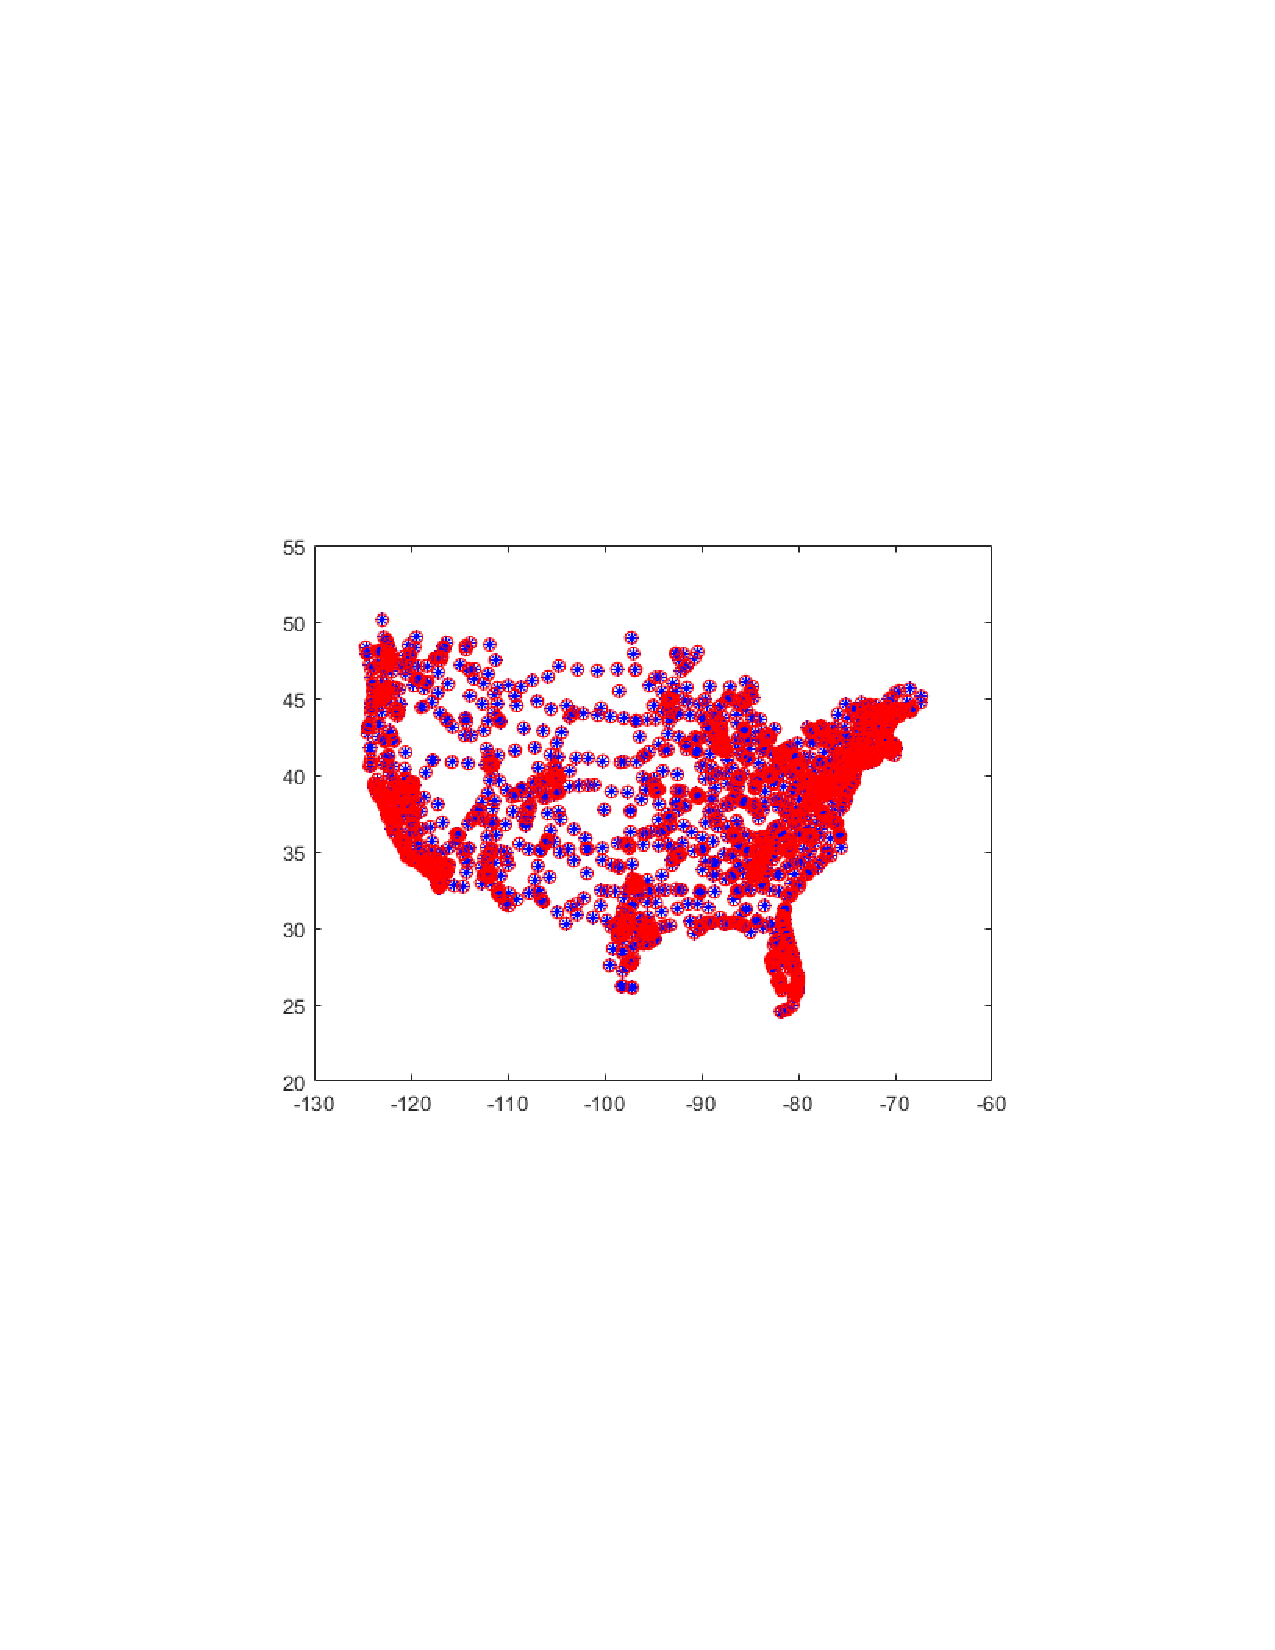
\includegraphics[width=3.2in]{charger_distribution.pdf}
%\vspace{-0.1in}
\caption{The Distribution of Charger Stations in US.}
\label{fig_charger_distribution}
%\vspace{-0.2in}
\end{figure}

\begin{figure}[!t]
\centering
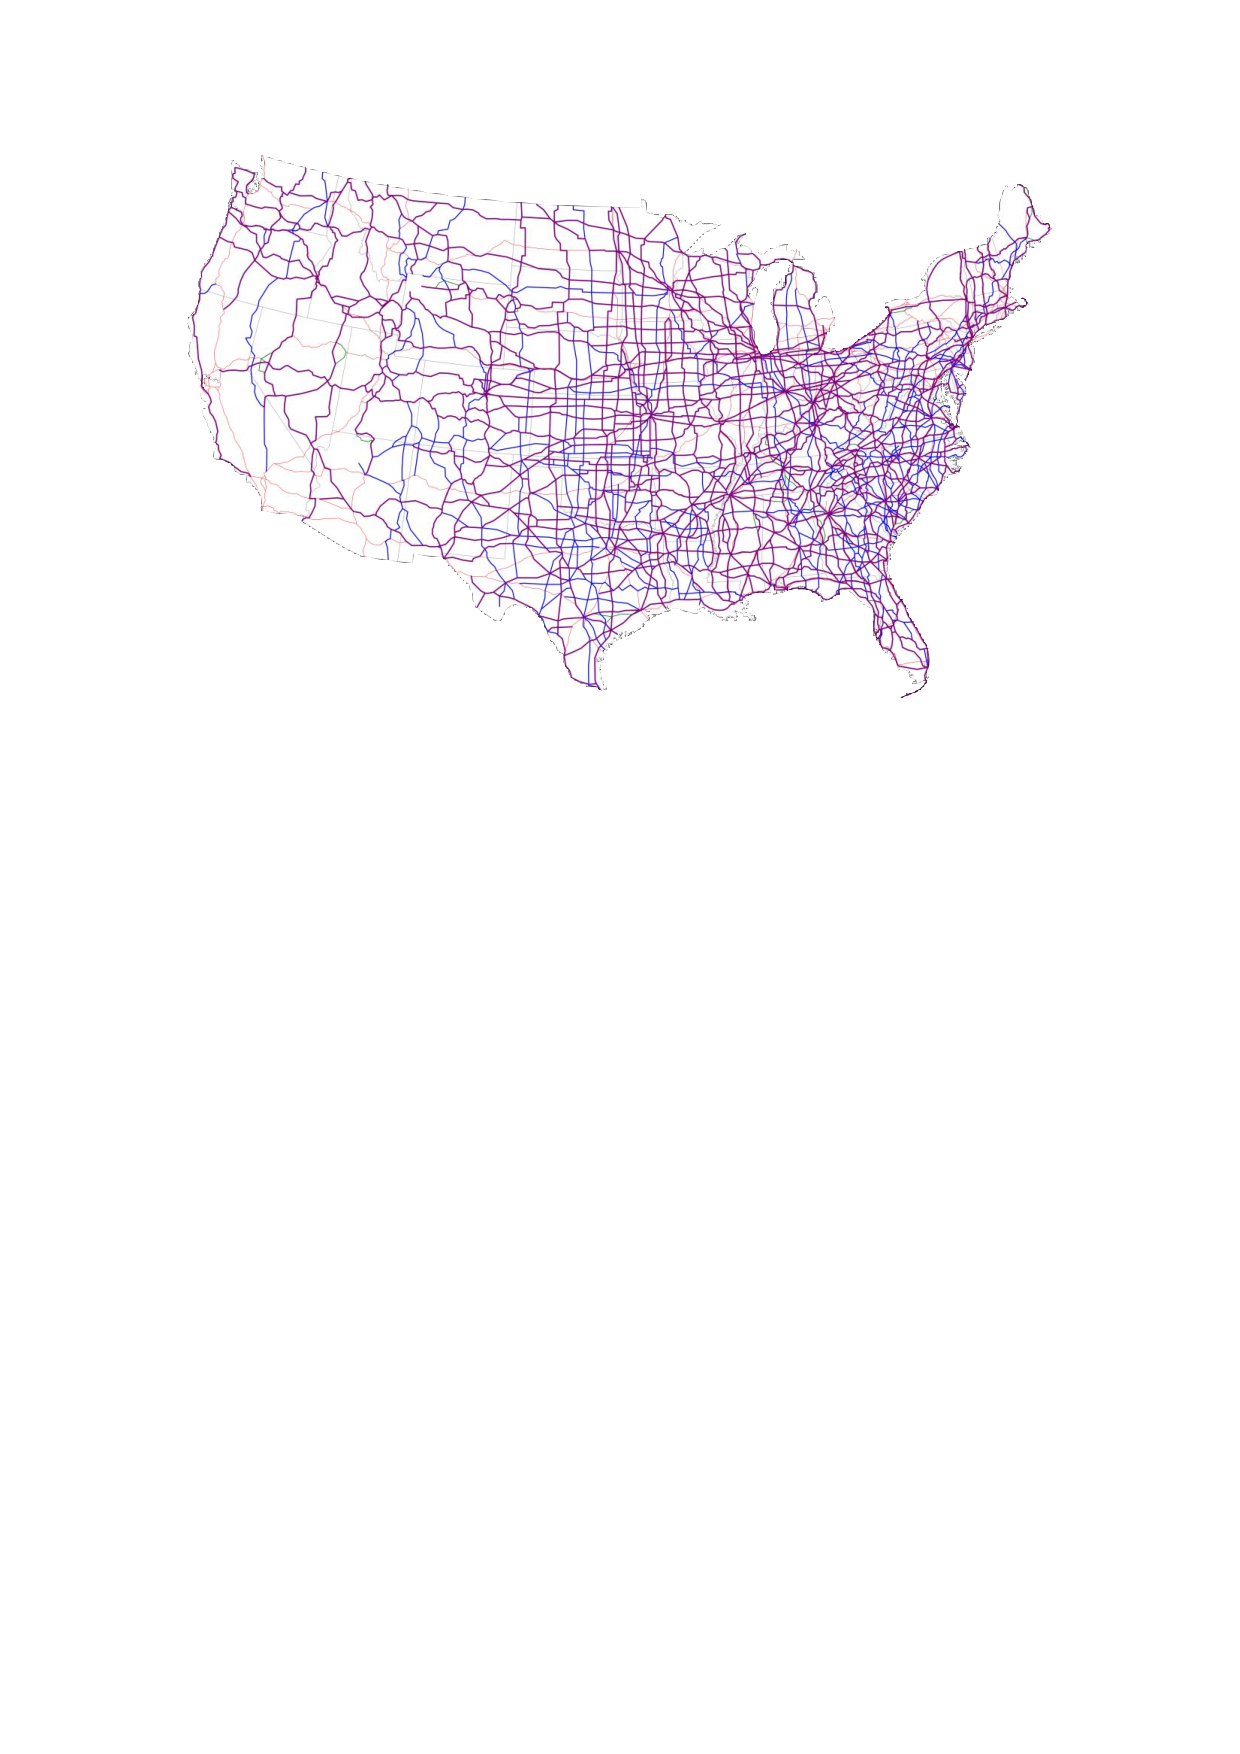
\includegraphics[width=3.2in]{road_map_us.pdf}
%\vspace{-0.1in}
\caption{The Road Map in US.}
\label{fig_road_map}
%\vspace{-0.2in}
\end{figure}

By analysing those data above, we can get three conclusions:
\begin{conclusion}
\label{conclusion_1}
Because of the density of roads, Tesla prefers to construct super charging stations in the area with low density of roads and destination charging station in the area with high density of roads.
\end{conclusion}
\begin{conclusion}
\label{conclusion_2}
As for features of various areas (\eg. urban, suburban, rural area......), Tesla prefers to more super charging stations in suburban and rural area and more destination charging stations in urban.
\end{conclusion}
\begin{conclusion}
\label{conclusion_3}
Tesla plans to deploy more super charging station in area of suburban in the future.
\end{conclusion}

\subsection{The Type of Charging Station}
According to the data above,
A charging station can be seen as a point with four kinds of attributes $sta(x, y, type, R)$.
Specifically, $x$, $y$ are the longitude and latitude of that charging station respectively.
$type$ is its charging type (\eg, destination charging, supercharging),
and $R$ is the maximum driving range provided by $sta(x, y, type, R)$.

Considering supercharging station case,
we find it can provide up to $170$ miles of range~\cite{SuperRange},
so we have $R_{super} = 170miles \approx 272km$.

As for the type of destination charging station,
we consider that it can provide the maximum driving range for an electric vehicle.
Thus, $R_{destination}$ depends on the type of the car.
To simplify our model, withou loss of generality, we assume that our target car is "Tesla Model 3"~\cite{CarRange}.
Considering "Tesla Model 3", the standard maximum range of it is $350km$,
so we have $R_{destination} = 350km$.
As a result, we have:
\begin{equation}
\label{equ_R}
\left\{
\begin{aligned}
& R_{super} = 272km \\
& R_{destination} = 350km \\
\end{aligned}
\right.
\end{equation}

\subsection{The Evaluation of US's Charging Station Network }
To evaluate whether Tesla can support the nation-wide migration of personal transportation to all-electric cars in the United States,
we need to first determine the conditions of a successful migration to all-electric vehicles in the United States.

Note that if the charging stations network can support a successful migration,
an electric vehicle must can get to another charging station from the location of a specific charging station,
so that it would not be restricted in certain area and can travel to anywhere of the whole expected reachable area.

Based on this idea, we can give the conditions of a successful migration to all-electric vehicles in the United States.
\begin{definition}
\label{def_successful_condtion}
\textbf{Successful Switch Condition:}
Suppose that the network of a target area $a$ can support a successful migration to all-electric vehicles,
then for every charing station $sta(x, y, type, R)$ in the network,
it can travel to any other charging station in this network.
\end{definition}

We can model the network as a graph $G_{a}(Vertex, Edge)$.
The set of vertexes $Vertex$ consists of the sites of charing stations.
For a specific site $i$, other sites $j$ that meet the distance $d(i,j) \leqslant R_{type}$ should have an edge $(i,j)$ between them.
All the edge form the set $Edge$.
and the value of a edge can be quantified as the distance.
With Definition~\ref{def_successful_condtion},
it can be considered as the \textbf{Connectivity of the Graph}~\cite{connectivity},
which means if the $G_{a}(Vertex, Edge)$ of area $a$ is a \textbf{Strongly Connected Graph},
then it can support a successful migration to all-electric vehicles in $a$.

Applying the analysis above,
the original problem is now the same as identifying whether the charging station graph $G_{US}(Vertex, Edge)$ of US is a Strongly Connected Graph.
Applying the classic algorithm related to Strongly Connected Graph~\cite{connectivity_algo},
we can reach the conclusion.
\subsubsection{The Result of Evaluation}
By our calculation, note that \textbf{the charging station network in US cannot support a complete switch to all electric}.
The reason of failure is the existence of the kind of case showed in Figure~\ref{fig_failure_case}.
Because $R_{destination} \geq R_{super}$,
there must exists the failure case that the electric vehicle can travel to a super charger station $i$ from a destination charger station $j$, but cannot get back to $j$ from $i$.
Thus, the charing stations network cannot be the Strongly Connected Graph.

In the result of our calculation,
note that there are around 92 this kind of failure in the network,
especially in area between the urban and suburban.
We propose the improvement solution to eliminate this kind of cases showed in Figure~\ref{fig_failure_case}.
Based on the improvement,
we evaluate that \textbf{the total number of charging station that can support a complete switch to all electric is around 3792},
which is higher than the number of current deployment.

\begin{figure}[!t]
\centering
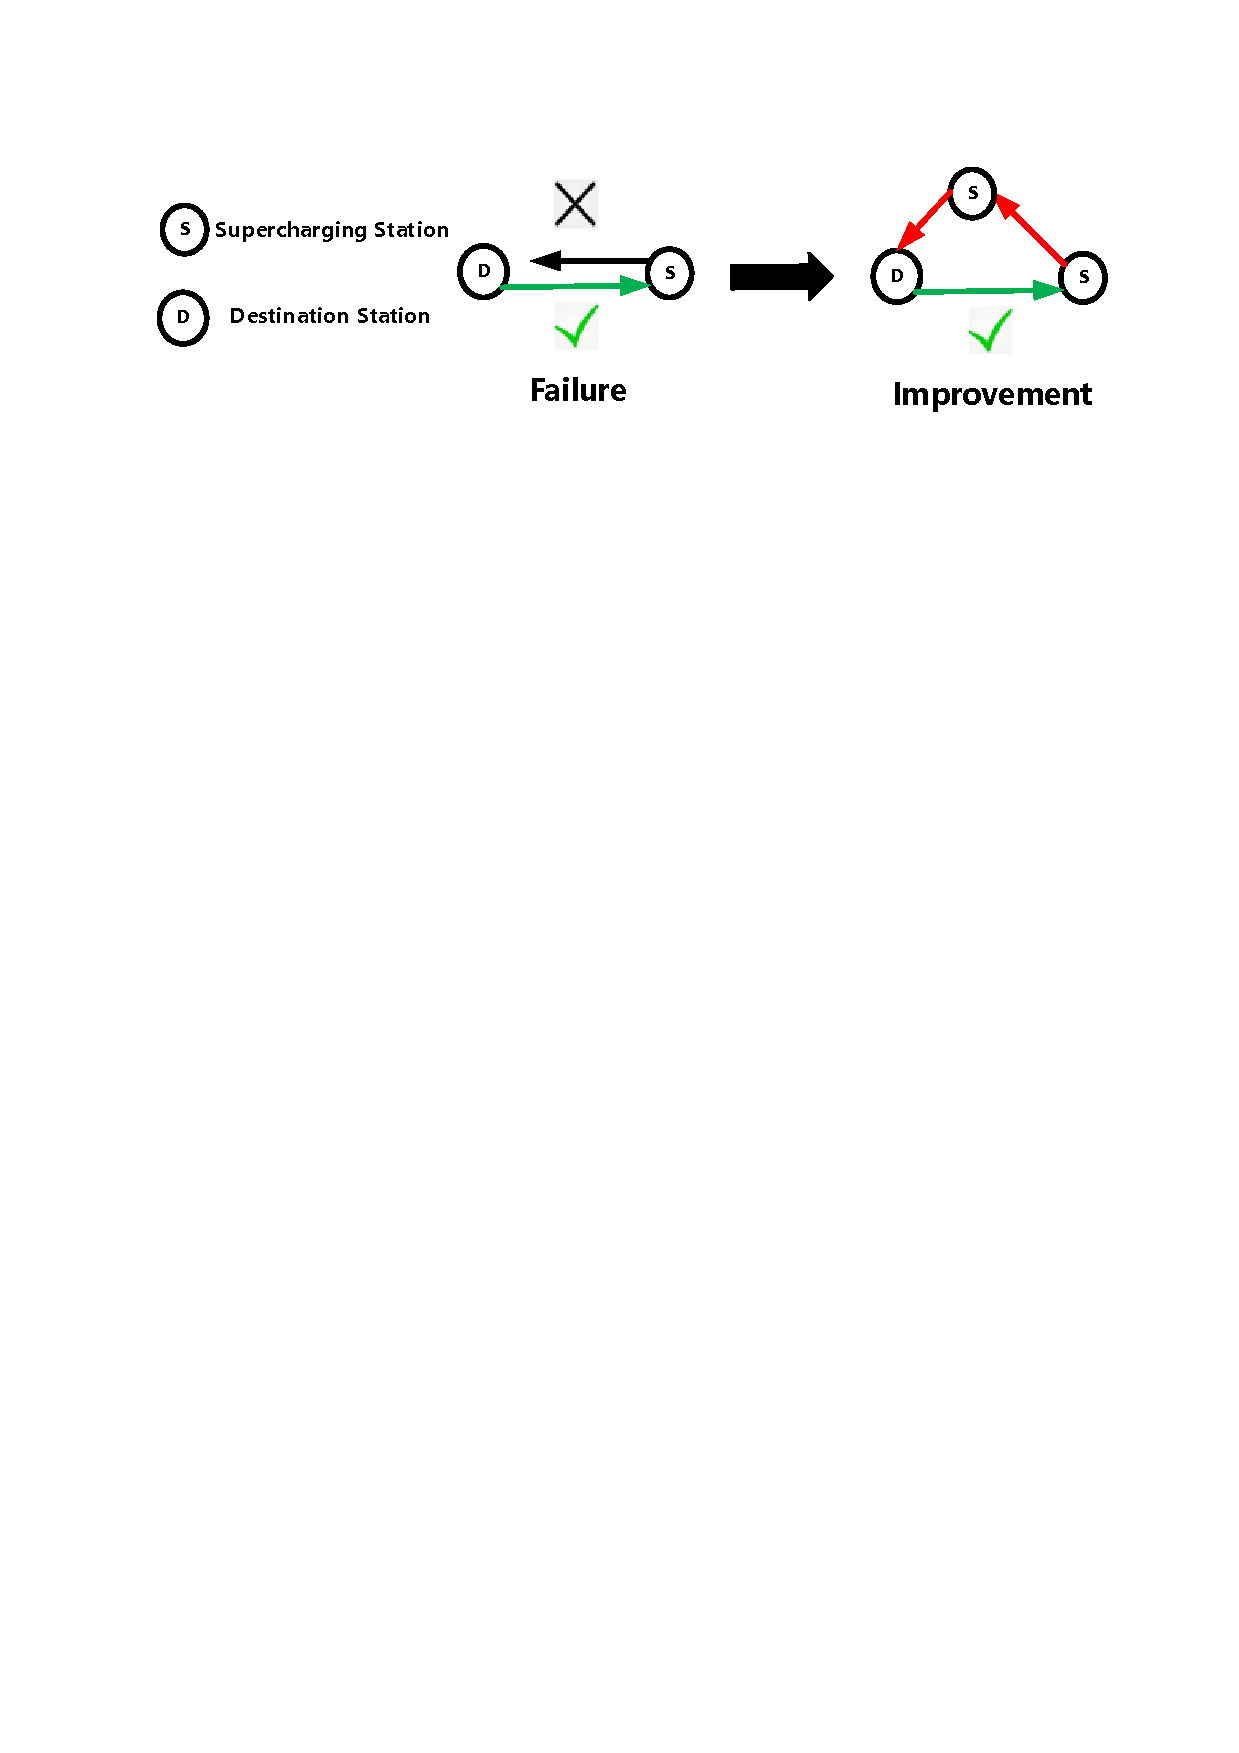
\includegraphics[width=5.2in]{failure_case.pdf}
%\vspace{-0.1in}
\caption{The Case of Failure and Improvement.}
\label{fig_failure_case}
%\vspace{-0.2in}
\end{figure}
